\documentclass{article}[18pt]
\ProvidesPackage{format}
%Page setup
\usepackage[utf8]{inputenc}
\usepackage[margin=0.7in]{geometry}
\usepackage{parselines} 
\usepackage[english]{babel}
\usepackage{fancyhdr}
\usepackage{titlesec}
\hyphenpenalty=10000

\pagestyle{fancy}
\fancyhf{}
\rhead{Sam Robbins}
\rfoot{Page \thepage}

%Characters
\usepackage{amsmath}
\usepackage{amssymb}
\usepackage{gensymb}
\newcommand{\R}{\mathbb{R}}

%Diagrams
\usepackage{pgfplots}
\usepackage{graphicx}
\usepackage{tabularx}
\usepackage{relsize}
\pgfplotsset{width=10cm,compat=1.9}
\usepackage{float}

%Length Setting
\titlespacing\section{0pt}{14pt plus 4pt minus 2pt}{0pt plus 2pt minus 2pt}
\newlength\tindent
\setlength{\tindent}{\parindent}
\setlength{\parindent}{0pt}
\renewcommand{\indent}{\hspace*{\tindent}}

%Programming Font
\usepackage{courier}
\usepackage{listings}
\usepackage{pxfonts}

%Lists
\usepackage{enumerate}
\usepackage{enumitem}

% Networks Macro
\usepackage{tikz}


% Commands for files converted using pandoc
\providecommand{\tightlist}{%
	\setlength{\itemsep}{0pt}\setlength{\parskip}{0pt}}
\usepackage{hyperref}

% Get nice commands for floor and ceil
\usepackage{mathtools}
\DeclarePairedDelimiter{\ceil}{\lceil}{\rceil}
\DeclarePairedDelimiter{\floor}{\lfloor}{\rfloor}

% Allow itemize to go up to 20 levels deep (just change the number if you need more you madman)
\usepackage{enumitem}
\setlistdepth{20}
\renewlist{itemize}{itemize}{20}

% initially, use dots for all levels
\setlist[itemize]{label=$\cdot$}

% customize the first 3 levels
\setlist[itemize,1]{label=\textbullet}
\setlist[itemize,2]{label=--}
\setlist[itemize,3]{label=*}

% Definition and Important Stuff
% Important stuff
\usepackage[framemethod=TikZ]{mdframed}

\newcounter{theo}[section]\setcounter{theo}{0}
\renewcommand{\thetheo}{\arabic{section}.\arabic{theo}}
\newenvironment{important}[1][]{%
	\refstepcounter{theo}%
	\ifstrempty{#1}%
	{\mdfsetup{%
			frametitle={%
				\tikz[baseline=(current bounding box.east),outer sep=0pt]
				\node[anchor=east,rectangle,fill=red!50]
				{\strut Important};}}
	}%
	{\mdfsetup{%
			frametitle={%
				\tikz[baseline=(current bounding box.east),outer sep=0pt]
				\node[anchor=east,rectangle,fill=red!50]
				{\strut Important:~#1};}}%
	}%
	\mdfsetup{innertopmargin=10pt,linecolor=red!50,%
		linewidth=2pt,topline=true,%
		frametitleaboveskip=\dimexpr-\ht\strutbox\relax
	}
	\begin{mdframed}[]\relax%
		\centering
		}{\end{mdframed}}



\newcounter{lem}[section]\setcounter{lem}{0}
\renewcommand{\thelem}{\arabic{section}.\arabic{lem}}
\newenvironment{defin}[1][]{%
	\refstepcounter{lem}%
	\ifstrempty{#1}%
	{\mdfsetup{%
			frametitle={%
				\tikz[baseline=(current bounding box.east),outer sep=0pt]
				\node[anchor=east,rectangle,fill=blue!20]
				{\strut Definition};}}
	}%
	{\mdfsetup{%
			frametitle={%
				\tikz[baseline=(current bounding box.east),outer sep=0pt]
				\node[anchor=east,rectangle,fill=blue!20]
				{\strut Definition:~#1};}}%
	}%
	\mdfsetup{innertopmargin=10pt,linecolor=blue!20,%
		linewidth=2pt,topline=true,%
		frametitleaboveskip=\dimexpr-\ht\strutbox\relax
	}
	\begin{mdframed}[]\relax%
		\centering
		}{\end{mdframed}}
\lhead{Networks and Systems - Compiler Design}


\begin{document}
\begin{center}
\underline{\huge Lexical Analysis}
\end{center}
The role of a lexical analyser
\begin{itemize}
	\item The first phase of a compiler
	\item Reads input characters
	\item Groups them into lexemes
	\item Produces as output a sequence of tokens
	\item The stream of tokens is sent to the parser
	\item When it discovers the lexeme for a new identifier it enters this lexeme into the symbol table
\end{itemize}
\subsection{Lexical Analysis vs Parsing}
Lexical analysis and syntax analysis are separate phases
\begin{itemize}
	\item Simplicity of design
	\begin{itemize}
		\item Simplify each task separately
	\end{itemize}
	\item Improved compiler efficiency
	\begin{itemize}
		\item Apply specialised techniques for each step
	\end{itemize}
	\item Compiler portability
	\begin{itemize}
		\item Different lexical analysers for specific devices
	\end{itemize}
\end{itemize}
\section{Tokens vs Lexemes}
Token
\begin{itemize}
	\item A notation representing the kind of lexical unit, e.g.
	\begin{itemize}
		\item A keyword
		\item An identifier
	\end{itemize}
	\item Consists of a pair of:
	\begin{itemize}
		\item A token name
		\item An (optional) attribute value
	\end{itemize}
	\item The tokens are given as input to the parser
\end{itemize}
Pattern of a token
\begin{itemize}
	\item A description of the form of its lexemes, e.g.
	\begin{itemize}
		\item For a keyword, the sequence of its characters
		\item For an identifier: a description that matches many strings
	\end{itemize}
\end{itemize}
The lexeme of a token
\begin{itemize}
	\item A sequence of characters in the source program that matches the pattern of the token
	\item The lexical analyser identifies a lexeme as an instance of a token
\end{itemize}
\section{Attributes of tokens}
In cases when many lexemes match with a specific token
\begin{itemize}
	\item The compiler must know which lexeme was found in the source program
	\item The lexical analyser provides to the parser
	\begin{itemize}
		\item The token name
		\item Additional information that specifies the particular lexeme represented by the token (attribute value)
	\end{itemize}
\end{itemize}
Token names - influence parsing decisions\\
\\
Attribute names - influence the transition of the token after the parsing (in the semantic analysis)\\
\\
Identifiers(token name is id):
\begin{itemize}
	\item Its lexeme (i.e. the sequence of its characters)
	\item Its type (e.g. integer, float, boolean)
	\item The line of the source program it has been found(in order to report error messages)
	\item etc
\end{itemize}
All this information is stored in the symbol table
\section{Recognition of tokens}
The source program can have several keywords:
\begin{itemize}
	\item e.g. if, then, else, for
	\item They are reserved words, i.e. can not be used as identifiers
	\item Their tokens have no attribute value
\end{itemize}
Patterns of tokens can be:
\begin{itemize}
	\item Expressed by regular expressions
	\item Defined by regular definitions (i.e. no recursive definitions)
\end{itemize}
Syntax of a program can be expressed by a context free grammar\\
\\
A simple context free grammar for branching statements:
\begin{center}
	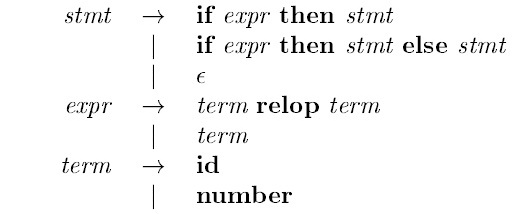
\includegraphics[scale=0.5]{context-free-grammar}
\end{center}
Terminal symbols of the grammar:
\begin{itemize}
	\item The token names, e.g. if, then, else, relop, id, number
	\item number: a "constant"; relop: for a "comparison operator"
\end{itemize}
Regular definitions for these operators
\begin{center}
	\includegraphics[scale=0.5]{"regular definitions"}
\end{center}
Important notes:
\begin{itemize}
	\item A superscript + means one or more
	\item A superscript * means zero or more
	\item A question mark at the end of brackets means optional
\end{itemize}
There is also an additional rule for stripping out whitespace
$$ws\rightarrow (\text{ blank }|   \text{ tab }  |  \text{ newline } )$$
All tokens with their attribute value and their corresponding lexemes
\begin{center}
	\includegraphics[scale=0.5]{"attribute value"}
\end{center}
\section{Transition diagrams}
\begin{itemize}
	\item When we scan the source diagram to identify lexemes, we need two pointers
	\begin{itemize}
		\item \texttt{lexemeBegin}: marks the beginning of the current lexeme
		\item \texttt{forward}: scans ahead until a pattern match is found
	\end{itemize}
	\item Patterns for tokens can be
	\begin{itemize}
		\item Expressed by regular expressions, and thus
		\item Recognised by a DFA
	\end{itemize}
	\item We model the recognition of a pattern by a transition diagram (a special type of a DFA)
	\begin{itemize}
		\item States represent all the current information between \texttt{lexemeBegin} and \texttt{forward}
		\item Actions are attached to the final states (to be performed after the lexeme has been scanned)
	\end{itemize}
	\item Types of actions attached to the final states:
	\begin{itemize}
		\item Return a specific token name and attribute value
		\item Retract the forward pointer one position (indicated by an *)
		\item Just proceed to the next character (for empty spaces),etc
		\item This is an example of a transition diagram for the token relop
	\end{itemize}
\end{itemize}
\begin{center}
	\includegraphics[scale=0.5]{"transition diagram"}
\end{center}
\section{Keywords vs Identifiers}
\begin{itemize}
	\item Keywords like for, if then else are reserved words and so can't be declared as identifiers even though they look like identifiers
	\item Usually we look for identifier lexemes with a transition diagram
	\begin{center}
		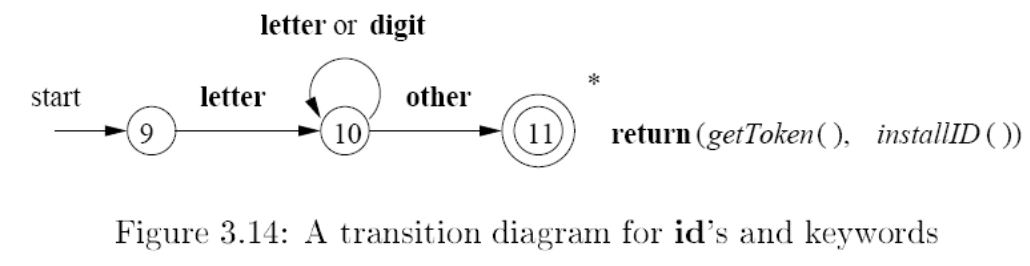
\includegraphics[scale=0.4]{lexemes}
	\end{center}
	
\end{itemize}
Two ways to handle reserved words:
\begin{enumerate}
	\item Install the reserved words initially in the symbol table, then:
	\begin{itemize}
		\item The corresponding entry in the symbol table stored information that this is a reserved word
		\item When we scan a lexeme, a call to installID
		\begin{itemize}
			\item Checks in the symbol table whether this lexeme is a reserved word
			\item It adds it in the symbol table (as an id) only if its not already there
		\end{itemize}
	\end{itemize}
	\item Create separate transition diagrams for each reserved word, example for then
	\begin{center}
		\includegraphics[scale=0.4]{"reserved word"}
	\end{center}
	\begin{itemize}
		\item We must check that the scanned word ends after reading then, otherwise it might be an identifier containing the word then
		\item For each new lexeme:
		\begin{itemize}
			\item First run the transition diagrams for reserved words
			\item If no accepts, the token can be recognised as id
		\end{itemize}
	\end{itemize}
		
\end{enumerate}
\section{Pattern Matching}
There exist tools to automatically generate a lexical analyser just by specifying the regular expressions to describe patterns to tokens\\
\\
An example of this is Lex, it performs as follows:
\begin{itemize}
	\item Lists some patterns (regular expressions) with some order
	\item Scans the input
	\begin{itemize}
		\item Until it finds the longest prefix of the input that matches one of the patterns
		\item If it matches many patterns, it chooses the first one in the order
	\end{itemize}
	\item Returns the corresponding token to the parser
\end{itemize}
Suppose Lex has three patterns\\
\begin{center}
	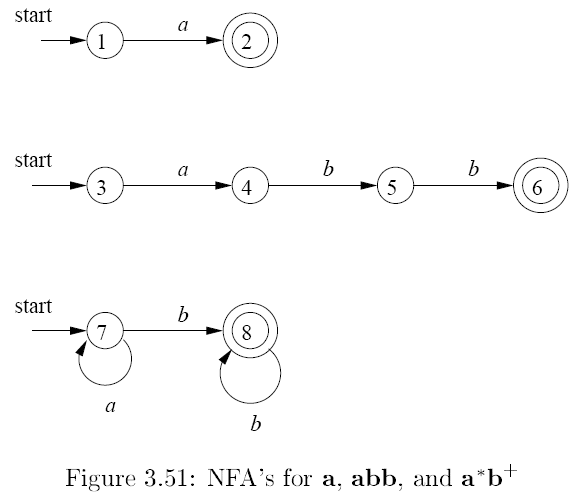
\includegraphics[scale=0.7]{recognise}
\end{center}
It composes a single equivalent NFA that recognises all of them
\begin{center}
	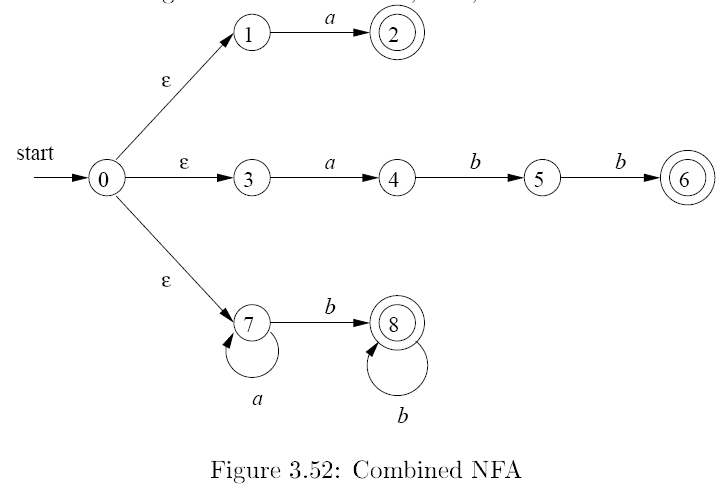
\includegraphics[scale=0.7]{combined}
\end{center}
As it moves ahead:
\begin{itemize}
	\item It calculates the set of states it is at each point
	\item It simulates the NFA until there are no next states
	\item After that:
	\begin{itemize}
		\item There can not be any longer prefix
		\item It looks backward, until it finds a set of states that includes a final state
		\item It picks the accepting state associated with the earliest pattern
		\item It returns this pattern
	\end{itemize}
\end{itemize}





\end{document}